\documentclass[student, noshadow, lsr, english, aspectratio=169, t]{ITR_LSR_slides}

\setbeamertemplate{frametitle}{%
  \vspace{0.3cm}% Space between top edge and title
  \if@center
    \begin{centering}
      \textbf{\vphantom{Sp}\insertframetitle\vphantom{Sp}}
      \par
    \end{centering}
  \else
    \textbf{\vphantom{Sp}\insertframetitle\vphantom{Sp}}
    \par
  \fi
  \vspace{0.3cm}% Space between title and content
}

% Add top margin to frames without titles
\addtobeamertemplate{frame begin}{%
  \ifx\insertframetitle\@empty
    \vspace{0.8cm}% Space at top of frames without titles
  \fi
}{}

\addbibresource{ref.bib}
\graphicspath{{pics/}{logos/}}

\title{Analysis and Control of Time-Varying and Perturbed Systems}
\presenter{Keno Bürger}
\typeofpres{Advanced Nonlinear Control}

\usepackage{multirow}
\usepackage{graphicx}
\usepackage[T1]{fontenc}
\usepackage{lmodern}
\usepackage{tabularx}
\usepackage{enumitem}
\usepackage{adjustbox}
\usepackage{booktabs}
\usepackage{makecell}
\PassOptionsToPackage{most}{tcolorbox}
\usepackage{tcolorbox}
\usepackage{amsmath,amssymb}
\usepackage{amsmath,amssymb}
\usepackage{hyperref}

% Load hyperref as the last package before document begins
\hypersetup{
	pdftitle={Advanced Nonlinear Control: Lyapunov Stability and Perturbations},
	pdfauthor={Keno Bürger},
	pdfsubject={Nonlinear Control Theory},
	pdfkeywords={Lyapunov stability, exponential stability, boundedness, ultimate boundedness, perturbations, nonlinear control},
	pdfcreator={LaTeX with Beamer},
	pdfproducer={pdfTeX},
}

% \newtcolorbox{assumptionbox}[1]{
% 	colback=blue!70!black, % Background color for the title part
% 	colframe=blue!70!black, % Frame color (same as background for a solid bar)
% 	coltext=white, % Text color for the title
% 	fonttitle=\bfseries, % Font for the title
% 	arc=3mm, % Rounded corners
% 	outer arc=3mm, % Rounded outer corners
% 	boxsep=2pt, % Space between the box content and the frame
% 	left=10pt, right=10pt, top=5pt, bottom=5pt, % Padding around title
% 	% Define the lower part with white background
% 	after title={\par\nobreak\vskip 5pt%
% 		\tcbset{
% 			colback=white, % Background color for the content part
% 			colframe=blue!70!black, % Frame color for the content part
% 			coltext=black, % Text color for the content part
% 			arc=3mm, % Rounded corners
% 			outer arc=3mm, % Rounded outer corners
% 			bottom=10pt, % Padding below content
% 			top=10pt, % Padding above content
% 			left=10pt, right=10pt, % Padding left and right
% 			sharp corners=south, % Make bottom corners sharp if you want to emphasize separation, or keep rounded for full rounded box
% 			rounded corners=southwest, rounded corners=southeast % Ensure only bottom corners are rounded
% 			}
% 		\begin{tcolorbox}
% 	},
% 	after upper={\end{tcolorbox}\nointerlineskip}, % Close the inner tcolorbox
% 	title={\parbox{\dimexpr\linewidth-20pt\relax}{#1}} % Title content
% }

% Fix for potential BOM or invisible characters
\begin{document}

\begin{frame}
    \titlepage
\end{frame}


%%%%%%%%%%%%%%%%%%%%%%%%%%%%%%%%%%%%%%%%%%%%%%%%%%%%%%
\section{Motivation}

\begin{frame}{Why Study Time-Varying Perturbed Systems?}
	\begin{itemize}
		\item \textbf{Real-World Imperfections:}
		\begin{itemize}
			\item Systems rarely time-invariant
			\item Parameters drift, components age, environment shifts
			\item \textit{Ex:} Aircraft dynamics change with fuel, altitude, air density
		\end{itemize}
		\item \textbf{Uncertainty Omnipresent:}
		\begin{itemize}
			\item External disturbances (wind gusts, load variations) inherent
			\item Internal uncertainties (sensor noise, actuator inaccuracies, unmodeled dynamics) ever-present
			\item \textit{Ex:} Robot arm payload or joint friction varies
		\end{itemize}
		\item \textbf{Performance \& Robustness Demands:}
		\begin{itemize}
			\item Modern control needs high performance (precision, speed) and robust stability
			\item Ignoring variations $\rightarrow$ poor performance, instability, failure
		\end{itemize}
	\end{itemize}
\end{frame}

\begin{frame}
    \frametitle{Understanding Perturbation Types}

    \textbf{Motivation:} Real-world systems exhibit time-dependence, modeling errors, external disturbances

    \vspace{0.5cm}
    \textbf{General System Form:}
    \[\dot{\underline{x}} = f(\underline{x}) + g(\underline{x}, t)\]

	\vspace{-0.5em}
    \begin{columns}[t,totalwidth=\textwidth]
        \column{0.48\textwidth}
		\begin{tcolorbox}[title=Vanishing Perturbation:]
			% \textbf{Vanishing Perturbation:}
			\begin{itemize}
				\item $g(\underline{x}, t) \to 0$ as $\underline{x} \to 0$.
				\item Preserves exponential stability.
				\item Examples: modeling errors, unmodeled dynamics
			\end{itemize}
		\end{tcolorbox}

        \column{0.48\textwidth}
        \begin{tcolorbox}[title=Non-Vanishing Perturbation:]
			\begin{itemize}
				\item $g(\underline{x}, t) \not\to 0$ as $\underline{x} \to 0$.
				\item Leads to ultimate boundedness.
				\item Examples: constant disturbances, sensor noise
			\end{itemize}
		\end{tcolorbox}
    \end{columns}
\end{frame}

% \begin{frame}
%     \frametitle{Main Objective}

%     \textbf{Based on:}
%     \begin{itemize}
%         \item \textit{Nonlinear Control} (Ch. 4): Time-varying and perturbed systems
%         \item \textit{Nonlinear Systems} (Ch. 9, 11.5): Stability under perturbations
%     \end{itemize}
% 	\vspace{0.5cm}
%     \textbf{Objective:}
%     \begin{itemize}
% 		\item Formulate practical and broadly applicable stability conditions
%         \item Analyze stability under \textbf{vanishing perturbations} using comparison functions
%         \item Study ultimate boundedness for systems with \textbf{non-vanishing perturbations}
%         % \item Apply Lyapunov-based methods for robust analysis of nonlinear, time-varying systems
%     \end{itemize}
% \end{frame}

%%%%%%%%%%%%%%%%%%%%%%%%%%%%%%%%%%%%%%%%%%%%%%%%%%%%%%
\section{Prerequisites}

\begin{frame}
	\frametitle{Lyapunov Theory for Time-Varying Systems}
	% \begin{itemize}
	% 	\item Definition of Uniform, Asymptotic and exponential stability \cite{muennighoff_s1_2025}
	% 	\item Application of Lyapunov Stability Theorems
	% \end{itemize}
	\textbf{Assumptions:}
	\begin{itemize}
		\item Origin $\underline{x}=0$ is an equilibrium point
		\item Lyapunov function $V(t,\underline{x})$ is continuously differentialbe, positive definite and radially unbounded
		\item Derivative of Lyapunov function is negative definite
	\end{itemize}
	\vspace{0.2cm}
	\begin{tcolorbox}[title=Globally uniformly exponentially stable:]
		\vspace{-0.4cm}
		\begin{align*}
			\exists\, c_i, \alpha > 0: & \; c_1\left\|\underline{x}\right\|^\alpha \leq V(t,\underline{x}) \leq c_2\left\|\underline{x}\right\|^\alpha  \\
			& \dot{V}(t,\underline{x}) \leq -c_3\|\underline{x}\|^\alpha
		\end{align*}	
	\end{tcolorbox}
	
\end{frame}

\begin{frame}
	\frametitle{Boundedness and Ultimate Boundedness}
	% \begin{itemize}
	% 	\item Differences
	% 	\item Build bridge to non vanishing and vanishing perturbations
	% \end{itemize}
	\begin{figure}
		\centering
		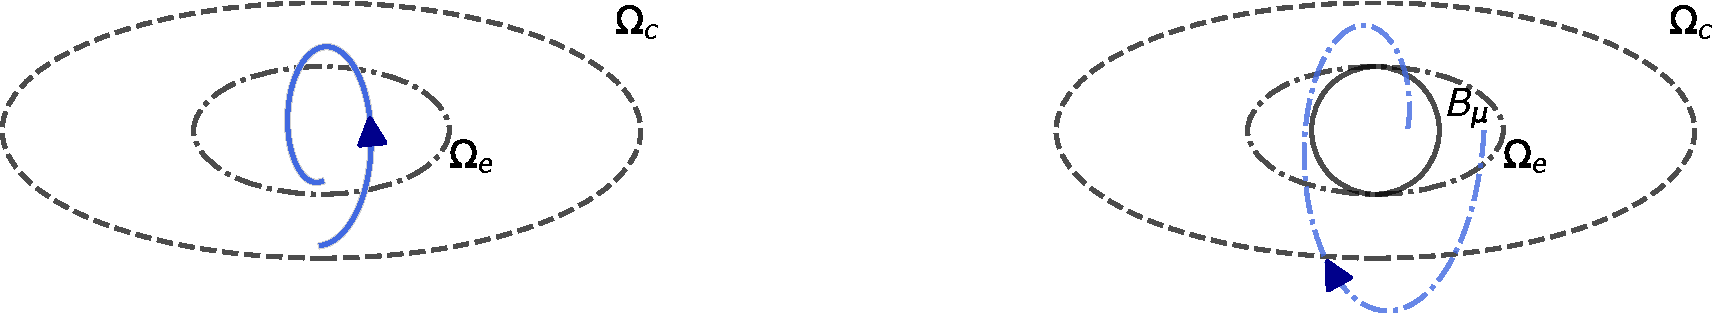
\includegraphics[width=\textwidth]{ultimate_boundedness_rotated.pdf}
		\caption{}
		\label{fig:boundedness_vs_ultimate_boundedness}
	\end{figure}
	\vspace{-2cm}
	\begin{columns}[t,totalwidth=\textwidth]
        \column{0.47\textwidth}
		\begin{tcolorbox}[title=Boundedness:]
			\vspace{-0.4cm}
			\begin{align*}
				\|\underline{x}(t_0)\| \leq \alpha \Rightarrow \|\underline{x}(t)\| \leq \beta,
				\\ c>0, \alpha\in(0,c),\, \beta>0,\,\forall\, t \geq t_0
			\end{align*}		
		\end{tcolorbox}
		
        \column{0.47\textwidth}
		\begin{tcolorbox}[title=Ultimate Boundedness:]
			\vspace{-0.4cm}
			\begin{align*}
				\|\underline{x}(t)\| \leq b 
				\\ \forall\, t \geq t_0+T
			\end{align*}
		\end{tcolorbox}
    \end{columns}
\end{frame}


%%%%%%%%%%%%%%%%%%%%%%%%%%%%%%%%%%%%%%%%%%%%%%%%%%%%%
\section{Vanishing Perturbations}

\begin{frame}
    \frametitle{Lyapunov Stability for Vanishing Perturbations}

    \textbf{Problem:} Analyze stability of $\dot{\underline{x}} = f(\underline{x}) + g(\underline{x}, t)$
    \begin{itemize}
        \item Nominal system ($\dot{\underline{x}} = f(\underline{x})$) exponentially stable
    \end{itemize}
	\vspace{0.3cm}
    \textbf{Assumptions for Exponential Stability:}
    \begin{itemize}
        \item Perturbation $g(\underline{x}, t)$ vanishes (i.e., $g(\underline{x}, t) \to 0$ as $\underline{x} \to 0$)
        \item $V(t,\underline{x})$: continuously differentialbe, positive definite, radially unbounded
    \end{itemize}
    \vspace{0.3cm} % Reduced vertical space
    \textbf{Condition for Global Uniform Exponential Stability:}
    \begin{align*}
        \frac{\partial V}{\partial t}+\frac{\partial V}{\partial \underline{x}}f(\underline{x}) &\leq -c_3\|\underline{x}\|^2 \text{ and } \left\|\frac{\partial V}{\partial \underline{x}}\right\| \leq c_4\|\underline{x}\| \\[0.5em]
        \|g(\underline{x},t)\| &\leq \gamma\|\underline{x}\| \text{ where } 0 \leq \gamma(t) < \frac{c_3}{c_4}
    \end{align*}

\end{frame}

\begin{frame}
    \frametitle{Comparison Lemma – Example}

	\vspace{-0.5cm}
	\begin{tcolorbox}[title=Problem: Analyze stability of a scalar perturbed system]
		\vspace{-0.4cm}
		\begin{align*}
			\dot{x} = -a\,x(t) + g(t, x), \quad x(0) = 0, \quad a > 0
		\end{align*}
	\end{tcolorbox}

    \textbf{Assumptions/Conditions:}
    \begin{itemize}
        \item $x(t) \geq 0 \quad \forall\, t \geq 0$.
        \item $g(t, x) \leq b\,x(t) \quad \forall\, x \geq 0$.
    \end{itemize}
	\vspace{0.3cm}
	\textbf{Integral Condition:}
	\begin{align*}
	\underline{x}(t) \leq \underline{x}_0 + \int_{t_0}^{t} \gamma(\tau)\, d\tau
	= \underline{x}_0 + \int_{t_0}^{t} [-a\,\underline{x}(\tau) + b\,\underline{x}(\tau)]\, d\tau
	\end{align*}
	\vspace{0.3cm}
	\textbf{Bound for Derivative:}
	\begin{align*}
	\dot{\underline{x}}(t) \leq -a\,\underline{x}(t) + b\,\underline{x}(t) = -(a - b)\,\underline{x}(t)
	\end{align*}
	\end{frame}
	
\begin{frame}
	\frametitle{Comparison Lemma – Example}
	\textbf{From the Bound for Derivative:}
	\begin{align*}
		\underline{x}(t) \leq \underline{x}_0 + \int_{t_0}^{t} \dot{\underline{x}}(\tau)\, d\tau
		\leq \underline{x}_0 - (a - b) \int_{t_0}^{t} \underline{x}(\tau)\, d\tau
	\end{align*}
	\vspace{0.3cm}
	\textbf{Note:} This applies if $(a-b)x$ is continuous, positive definite, and non-decreasing.
	\vspace{-0.3cm}
	\begin{tcolorbox}[title=Conclusion: Exponential Stability of the Perturbed System]
		\vspace{-0.4cm}
		\begin{align*}
			\lim_{t \to \infty} \underline{x}(t) = 0 \\[0.3cm]
			\underline{x}(t) \leq \underline{x}_0\, e^{-(a - b)t}
		\end{align*}
	\end{tcolorbox}
\end{frame}

%%%%%%%%%%%%%%%%%%%%%%%%%%%%%%%%%%%%%%%%%%%%%%%%%%%%%
\section{Non-Vanishing Perturbations}
\subsection*{Ultimate Boundedness} % Sub-section for navigation

\begin{frame}
    \frametitle{Non-Vanishing Perturbations: The Problem}
	\textbf{The Challenge:}
    \begin{itemize}
        \item Perturbation doesn't disappear, perfect asymptotic stability to zero is not possible
        \item State $\underline{x}$ will perpetually move away from the origin
    \end{itemize}

    \vspace{0.3cm}
    \textbf{Conclusion/Goal: Ultimate Boundedness}
    \begin{itemize}
        \item We aim for Ultimate Boundedness
        \item Not exactly zero, but "close enough" for practical purposes
    \end{itemize}

	\vspace{0.3cm}
    \textbf{Intuition:}
    \begin{itemize}
        \item Imagine balencing a pencil on its tip in a sufficiently strong wind
        \item It won't stay perfectly still
        \item Find out how big that wobble area is $\Rightarrow$ guarantee the pencil always stays inside
    \end{itemize}
\end{frame}

\begin{frame}
    \frametitle{Lyapunov Conditions for Ultimate Boundedness}

    \textbf{Given:}
    \begin{itemize}
        \item System $\dot{\underline{x}} = f(\underline{x}) + g(\underline{x}, t)$.
        \item Nominal system origin $\underline{x}=0$ exponentially stable.
    \end{itemize}
	\vspace{0.3cm}
	\textbf{Criteria (Assumptions \& Conditions):}
    \begin{itemize}
        \item \textbf{Lyapunov Function:} Cont. diff., pdf, radially unbounded
            %   \[c_1\|\underline{x}\|^2 \leq V(t,\underline{x}) \leq c_2\|\underline{x}\|^2\]
			%   \textit{Dummies: $V$ is like energy; positive means it's big away from origin, zero at origin.}
        \item \textbf{Nominal Decay Condition:} Derivative of $V$ along nominal system is ndf
            %   \[\frac{\partial V}{\partial t}+\frac{\partial V}{\partial \underline{x}}f(\underline{x}) \leq -c_3\|\underline{x}\|^2 \]
            %   \textit{Dummies: Nominal system's "energy" always decreases, pulling state towards origin.}
        \item \textbf{Lyapunov Function Gradient Bound:} Gradient of $V$ is bounded
            %   \[\left\|\frac{\partial V}{\partial \underline{x}}\right\| \leq c_4\|\underline{x}\|\]
            %   \textit{Dummies: How fast "energy" changes w.r.t. position; not too steep.}
        \item \textbf{Perturbation Bound:} Non-vanishing $g(\underline{x}, t)$ is bounded by a constant $\delta$
            %   \[\|g(\underline{x}, t)\| \leq \delta \]
            %   \textit{Dummies: External disturbance is noisy but has a finite maximum strength $\delta$.}
    \end{itemize}
	\vspace{0.3cm}
    \textbf{The Key Trade-off:} $\delta$ directly impacts size of ultimate bound
    \begin{align*}
		\|g(\underline{x}, t)\| \leq \delta < \frac{c_3}{c_4} \sqrt{\frac{c_1}{c_2}}\, \theta r, \quad \theta \in (0,1),\ r > 0
	\end{align*}

\end{frame}

\begin{frame}
    \frametitle{Result: Initial Decay and Ultimate Boundedness}
	\vspace{-0.5cm}
	\begin{tcolorbox}[title=Outcome for any initial condition $\|\underline{x}(t_0)\| \leq \sqrt{c_1/c_2} \, r$]
		\textbf{Phase 1: Initial Exponential Decay}
		\begin{align*}
			\underline{x}(t)\| \leq k\, e^{-\gamma (t - t_0)} \|\underline{x}(t_0)\|, \quad t_0 \leq t \leq t_0 + T
		\end{align*}
		\textbf{Phase 2: Ultimate Boundedness}
		\begin{align*}
			\underline{x}(t)\| \leq b \quad \forall\, t \geq t_0 + T
		\end{align*}
	\end{tcolorbox}
    \vspace{0.3cm}
    \textbf{What it Means:}
    \begin{itemize}
        \item $\underline{x}(t_0)$ sufficiently close to origin $\Rightarrow$ system initially heads towards origin rapidly
        \item Due to non-vanishing perturbation it will settle into ultimate around the origin
        \item $b$ depends directly on $\delta$ and how "stable" the system is ($c_1, c_2, c_3, c_4$)
    \end{itemize}

    % \vspace{0.3cm}
    % \textbf{Key Parameters:}
    % \[ k = \sqrt{\frac{c_2}{c_1}}, \quad \gamma = \frac{(1 - \theta)c_3}{2c_2}, \quad b = \frac{c_4}{c_3}k \frac{\delta}{\theta} \]
    % \textit{Dummies: These are like calibration numbers telling us how fast it decays ($k, \gamma$) and how big the final wobble will be ($b$).}
\end{frame}

\begin{frame}
    \frametitle{Example: Bounded Disturbance Response}
	\vspace{-0.5cm}
    \begin{tcolorbox}[title=Problem: Analyze Boundedness of a Perturbed Mass-Spring-Damper-System]
		\vspace{-0.4cm}
        \begin{align*}
            \dot{x}_1 &= x_2 \\ % Position
            \dot{x}_2 &= -2x_1 - 3x_2 + d
        \end{align*}
        with bounded disturbance $|d| \leq \delta$ and the origin of the nominal system being exponentially stable.
    \end{tcolorbox}

    \vspace{0.3cm}
    \textbf{Lyapunov Candidate Function:} $V(\underline{x}) = \underline{x}^T P \underline{x}$
    \begin{itemize}
        \item $P > 0$ found by solving $A^T P + P A = -Q$
        \item For $Q=I$ and $A = \begin{bmatrix} 0 & 1 \\ -2 & -3 \end{bmatrix}$, $P$ can be calculated
        \item $c_1 \|\underline{x}\|^2 \leq V(\underline{x}) \leq c_2 \|\underline{x}\|^2$.
    \end{itemize}

\end{frame}

\begin{frame}
    \frametitle{Example: Bounded Disturbance Response}

    \textbf{Applying Lyapunov Stability Conditions:}
		\[ \dot{V} \leq -c_3 \|\underline{x}\|^2 + c_4 \|d\| \|\underline{x}\| \leq -c_3 \|\underline{x}\|^2 + c_4 \delta \|\underline{x}\| \]

    % \vspace{0.3cm}
    % \textbf{Recalling Boundedness Condition:}
    % \begin{itemize}
    %     \item If $\delta$ satisfies the condition:
    %           \[ \delta < \frac{c_3}{c_4} \sqrt{\frac{c_1}{c_2}} \theta r, \quad \theta \in (0,1), r>0 \]
    %           (This ensures the "pull towards zero" is stronger than the "push from disturbance" outside a small ball.)
    % \end{itemize}

    \vspace{-0.1cm}
    \begin{tcolorbox}[title=Conclusion: Ultimate Boundedness Guaranteed]
        \begin{itemize}
            \item System state $\|\underline{x}(t)\|$ eventually converges to and remains within a bounded region:
                  \[ \|\underline{x}(t)\| \leq b \quad \forall\, t \geq t_0 + T \]
            \item The ultimate bound $b$ and other parameters are:
                  \[ b = \frac{c_4}{c_3} k \frac{\delta}{\theta}, \quad k = \sqrt{c_2/c_1}, \quad \gamma = \frac{(1 - \theta)c_3}{2c_2} \]
            \item Size of the ultimate bound $b$ directly \textbf{scales with the disturbance magnitude $\delta$}.
        \end{itemize}
    \end{tcolorbox}
\end{frame}


%%%%%%%%%%%%%%%%%%%%%%%%%%%%%%%%%%%%%%%%%%%%%%%%%%
\section{Summary and Discussion}

\begin{frame}
    \frametitle{Key Insights \& Practical Implications}

    \textbf{Theoretical Insights:}
    \begin{itemize}
        \setlength{\itemsep}{8pt}
        \item Lyapunov methods: unify time-varying and perturbed system analysis
        \item Perturbation type: dictates achievable stability properties
        \item Ultimate boundedness: models real-world robustness
    \end{itemize}

    \vspace{0.8cm}
    \textbf{Design Implications:}
    \begin{itemize}
        \setlength{\itemsep}{8pt}
        \item Small, vanishing perturbations: maintains exponential convergence
        \item Persistent disturbances: design for bounded operation
        \item Robustness: requires accurate perturbation characterization
    \end{itemize}
\end{frame}




%%%%%%%%%%%%%%%%%%%%%%%%%%%%%%%%%%%%%%%%%%%%%%%%%%%%%
\appendix

\begin{frame}[allowframebreaks]
    \frametitle{References}
    \nocite{*} 
    \printbibliography[heading=none]
\end{frame}

\end{document}
